\documentclass{sigchi}

% Use this section to set the ACM copyright statement (e.g. for
% preprints).  Consult the conference website for the camera-ready
% copyright statement.

% Copyright
% \CopyrightYear{2016}
% %\setcopyright{acmcopyright}
% \setcopyright{acmlicensed}
% %\setcopyright{rightsretained}
% %\setcopyright{usgov}
% %\setcopyright{usgovmixed}
% %\setcopyright{cagov}
% %\setcopyright{cagovmixed}
% % DOI
% \doi{http://dx.doi.org/10.475/123_4}
% % ISBN
% \isbn{123-4567-24-567/08/06}
% %Conference
% \conferenceinfo{CHI'16,}{May 07--12, 2016, San Jose, CA, USA}
% %Price
% \acmPrice{\$15.00}

% Use this command to override the default ACM copyright statement
% (e.g. for preprints).  Consult the conference website for the
% camera-ready copyright statement.

%% HOW TO OVERRIDE THE DEFAULT COPYRIGHT STRIP --
%% Please note you need to make sure the copy for your specific
%% license is used here!
% \toappear{
% Permission to make digital or hard copies of all or part of this work
% for personal or classroom use is granted without fee provided that
% copies are not made or distributed for profit or commercial advantage
% and that copies bear this notice and the full citation on the first
% page. Copyrights for components of this work owned by others than ACM
% must be honored. Abstracting with credit is permitted. To copy
% otherwise, or republish, to post on servers or to redistribute to
% lists, requires prior specific permission and/or a fee. Request
% permissions from \href{mailto:Permissions@acm.org}{Permissions@acm.org}. \\
% \emph{CHI '16},  May 07--12, 2016, San Jose, CA, USA \\
% ACM xxx-x-xxxx-xxxx-x/xx/xx\ldots \$15.00 \\
% DOI: \url{http://dx.doi.org/xx.xxxx/xxxxxxx.xxxxxxx}
% }

% Arabic page numbers for submission.  Remove this line to eliminate
% page numbers for the camera ready copy
% \pagenumbering{arabic}

% Load basic packages
\usepackage{balance}       % to better equalize the last page
\usepackage{graphics}      % for EPS, load graphicx instead
\usepackage[T1]{fontenc}   % for umlauts and other diaeresis
\usepackage{txfonts}
\usepackage[utf8]{inputenc}
\usepackage{mathptmx}
\usepackage[pdflang={en-US},pdftex]{hyperref}
\usepackage{color}
\usepackage{booktabs}
\usepackage{textcomp}

% Some optional stuff you might like/need.
\usepackage{microtype}        % Improved Tracking and Kerning
% \usepackage[all]{hypcap}    % Fixes bug in hyperref caption linking
\usepackage{ccicons}          % Cite your images correctly!
% \usepackage[utf8]{inputenc} % for a UTF8 editor only

% If you want to use todo notes, marginpars etc. during creation of
% your draft document, you have to enable the "chi_draft" option for
% the document class. To do this, change the very first line to:
% "\documentclass[chi_draft]{sigchi}". You can then place todo notes
% by using the "\todo{...}"  command. Make sure to disable the draft
% option again before submitting your final document.
\usepackage{todonotes}

% Paper metadata (use plain text, for PDF inclusion and later
% re-using, if desired).  Use \emtpyauthor when submitting for review
% so you remain anonymous.
\def\plaintitle{Our Paper Title}
\def\plainauthor{First Author, Second Author, Third Author,
  Fourth Author}
\def\emptyauthor{}
\def\plainkeywords{Authors' choice; of terms; separated; by
  semicolons; include commas, within terms only; required.}
\def\plaingeneralterms{Documentation, Standardization}

% llt: Define a global style for URLs, rather that the default one
\makeatletter
\def\url@leostyle{%
  \@ifundefined{selectfont}{
    \def\UrlFont{\sf}
  }{
    \def\UrlFont{\small\bf\ttfamily}
  }}
\makeatother
\urlstyle{leo}

% To make various LaTeX processors do the right thing with page size.
\def\pprw{8.5in}
\def\pprh{11in}
\special{papersize=\pprw,\pprh}
\setlength{\paperwidth}{\pprw}
\setlength{\paperheight}{\pprh}
\setlength{\pdfpagewidth}{\pprw}
\setlength{\pdfpageheight}{\pprh}

% Make sure hyperref comes last of your loaded packages, to give it a
% fighting chance of not being over-written, since its job is to
% redefine many LaTeX commands.
\definecolor{linkColor}{RGB}{6,125,233}
\hypersetup{%
  pdftitle={\plaintitle},
% Use \plainauthor for final version.
%  pdfauthor={\plainauthor},
  pdfauthor={\emptyauthor},
  pdfkeywords={\plainkeywords},
  pdfdisplaydoctitle=true, % For Accessibility
  bookmarksnumbered,
  pdfstartview={FitH},
  colorlinks,
  citecolor=black,
  filecolor=black,
  linkcolor=black,
  urlcolor=linkColor,
  breaklinks=true,
  hypertexnames=false
}

% create a shortcut to typeset table headings
% \newcommand\tabhead[1]{\small\textbf{#1}}

% End of preamble. Here it comes the document.
\begin{document}
\title{\plaintitle}
\numberofauthors{3}
\author{%
  \alignauthor{Leave Authors Anonymous\\
    \affaddr{for Submission}\\
    \affaddr{City, Country}\\
    \email{e-mail address}}\\
  \alignauthor{Leave Authors Anonymous\\
    \affaddr{for Submission}\\
    \affaddr{City, Country}\\
    \email{e-mail address}}\\
  \alignauthor{Leave Authors Anonymous\\
    \affaddr{for Submission}\\
    \affaddr{City, Country}\\
    \email{e-mail address}}\\
}

\maketitle

\begin{abstract}
  Smart Textiles and body worn controller (Wearables) have been analyzed, mostly individually, using different technologies and on different aspects. Although there were some tests concerning everyday life, they are not used very often in this situation life for several reasons. This paper aims to show some of them and analyze, instead, the opportunities that  may lead to a better development and improve the feeling that a user has when interacting in an uncommon way with a device. One of the main threats that this paper discuss will be the reasons for social unacceptability, methods to review social acceptability and possible solutions for the problems concerning the usage of Wearables in public minding also technology-related tradeoffs.
  To illustrate the issues different Wearables are going to be presented - specifically concentrating on the social aspects of the devices. Finally this paper discusses further development of social acceptability of Wearables in the future.
\end{abstract}
% \category{H.5.m.}{Information Interfaces and Presentation
%   (e.g. HCI)}{Miscellaneous} \category{See
%   \url{http://acm.org/about/class/1998/} for the full list of ACM
%   classifiers. This section is required.}{}{}
%
% \keywords{\plainkeywords}
%
% \section{Introduction} \label{test:intro}
%
% Here there's the intro.
% \\ \textbf{Bold text} is done with
% \begin{verbatim}
%   \textbf{Bold text}
% \end{verbatim}
% \emph{emphatized text} is done with
% \begin{verbatim}
%   \emph{emphatized text}
% \end{verbatim}
% New line is made with double backslash
% \begin{verbatim}
%   line \\ another line
% \end{verbatim}
% \subsection{A subsection}
% Text of the subsection is shown here.
% \subsubsection{This is a subsubsection}
% We should not go further in sub sectioning, so we shall not use \textit{paragraph} and \textit{subparagraph}
% % References must be the same font size as other body text.
\section{Introduction}
%
% quick overview over the topic. Philipp already mentioned that his abstract might be a good starting point.
% Also we should give an introduction on the respective parts of the paper and give reason for the research we did (why is social acceptability an issue…)

Touch gestures are a form of interaction that is used by almost everyone daily in our society. Whether Smartphone, Tablet or Smartwatch - many mobile devices are nowadays controlled by this input technique to master different tasks. High demands are attached to the fast and intuitive use of these devices. The combination of different electronic devices can help to achieve these requirements in a new measure. For example, smart watches are already used to control mobile phones or various home electronics (e.g. controlling lamps). The development of innovative input devices, which can be integrated into clothing or even applied to the user's skin, offers the potential to communicate with electronic devices in completely new ways and make interaction even more intuitive. Especially we focus on touch input devices that are attached to the user's skin or are integrated into clothing and can be used to control different electronic devices.

Because these technologies create new and unusual forms of interaction, we will also look on third-party perceptions of a user’s interactions with a wearable e-textile interface. Social conventions play an important role in the development of these new forms of interaction. The willingness to make gestures depends largely on how appropriate these actions look and feel in public. [Source: Don’t Mind me Touching my wrist] For example, interaction with a touch panel attached to the breast can be disgusting for some people. The usability of these technologies must also be considered. To support the user as efficiently, effectively and satisfactorily as possible, the designers must also consider the interaction with the system in addition to the placement of this body-worn controllers.



\section{Showcase of technology examples}

Maybe first a definition of body-worn controllers and a not, that we want to concentrate on Touch-Input.
I think it is a good idea to pick a few examples which were mentioned in the papers and discuss them briefly.
For the first part (just the showcase) it is sufficient to just write down the basic technology (with Source): So what it is? How does is work (very briefly)? What it is used for?
We can get more into detail in the pros/cons section below


In order to get a rough overview of the interaction possibilities with Body-worn controller, different existing approaches are shown in this section.

Augmented Reality related research is still trying to optimise the input, which interacts with the shown interface. This research area could potentially capitalize on the natural and unobtrusive ways you interact with Wearables.
“Belt” (Source paper on belt) is an Body-worn controller specifically build to interact with Augmented Reality applications. As the name suggests the device is worn around the hip, like a regular belt. The device is touch-sensitive and can differentiate between simple gestures and locate the position of the touch-input (Source Page 2136). One of the main use cases of the device are spatial mapped shortcuts to open apps, like a virtual wallet for example.

\section{Multi-Touch Skin: A thin and flexible Multi touch Sensor for On-Skin Input}
% also true for iSkin
A current approach deals with the placement of multi-touch sensors directly on the skin. Because the human body surface is differently curved and deformable, the system must be particularly flexible and adaptable to fit the skin. This is a special requirement for the design of the sensors as it needs to satisfy the comfort of the user wearing it, who should not feel the fact that he or she is wearing a sensor, and the necessity for the input to be fixed on a position of the body to recognize correctly the input, which requires tightness onto the skin. Furthermore, the human body has electrocapacitive effects, which must be correctly shielded from an input sensor to ensure reliable touch detection which places special demands on the technology's material: it must both be insulated by the conductive sweat produced by the skin, but it has to let the same sweat flow outside, to avoid the user to feel uncomfortable due to the impossibility of the the skin to dissipate the heat in that area.
%The material, moreover, should be elastic like the skin is, to avoid the user to feel %tightened and for the sensor to lose the capability to detect the input if it’s not tight %enough at any time.
To master these challenges, the researchers studied various materials and manufacturing processes. As a result of this research work, a multi-touch sensor was developed, which can be applied directly to the user's skin in form of a thin layer and thus adapts flexibly to the different body shapes. To counteract the capacitive properties of the human body, the prototype consists of three layers, the transmitting, receiving and shielding layer. The individual layers are produced using a standard printer. Silver ink was used here because silver is a particularly effective electrical conductor and so is perfectly qualified to produce the sensor units. Furthermore, this method is well suited to produce multi-touch sensors in different sizes and therefore to test them on different body regions.
Possible uses are:
A small multi-touch sensor behind the ear could be used to manipulate an audio device. For example, the user could adjust the volume by stroking the sensor or pause playback with a simple click. A wristband sized sensor could be used to control interactive lamps. Users could place two fingers around the wrist and rotate them to change the color of a light bulb or adjust the brightness of a lamp using swipe gestures.

Another solution is presented by iSkin [ref], where a different material is used to allow input to be sensed. The polydimethylsiloxane (PDMS), the silicon-based material used, is “fully transparent, elastic, and a highly biocompatible material. [...] Therefore it is widely used on or in the human body, for example in body implants.” PDMS is non-conductive, but adding carbon to it lead to cPDMS, which can create a conductive surface. This allows to create gray sensible surfaces with specific drawn theme on it, which can immediately let the user know what to press for an action, but it doesn’t allow gestures to be performed on, as the principle on which it’s build is an RC charge-discharge time evaluation of the sensible surface.

\section{e-Textiles}
E-textiles, the contraction of electronic textiles, are input devices fitted or integrated into the fabric of a user's clothing. These surfaces allow the user to interact with various electronic devices in his environment, as they integrates both the sensing surface, which takes the physical input like touch, grab or fingering,  and a control unit, which elaborate the input and send it to a controlled device. This means that usually an e-textile is only an input surface, which implies the necessity for the surface itself not to be rigid in order to let the skin act as a direct feedback for the user.

An example for e-Textiles is “Pinstripe” a project by the University Aachen. This technology is directly integrated in clothing by conductive threads. The threads measure folds, which are created by pinching the fabric with thumb and index finger. When the fold is rolled across the fabric the rolling gesture accompanied by the diameter of the fold acts as an input (smaller folds represent finer inputs). Those inputs can be used for example to manipulate the volume of a music player.

Another e-textile is the "Jogwheel", which was developed as part of the paper "Don't Mind Me Touching My Wrist: A Case Study of Interacting with On- Body Technology in Public" [X] to investigate the social acceptance of on-body technology. The jogwheel is visually comparable to a fabric patch and is made of conductive yarn. A tactile surface structure should guide the user's fingers, which simplifies eye-free interaction. The developers describe the size of the jogwheel as twice the size of the iPod click wheel. This size should allow high precision in use and several types of one-handed gestures. Figures N, M show the jog wheel and two ways of interaction with them. The e-Textil can be placed anywhere on the user's clothing for controlling electronic devices. [X]
\begin{figure}
  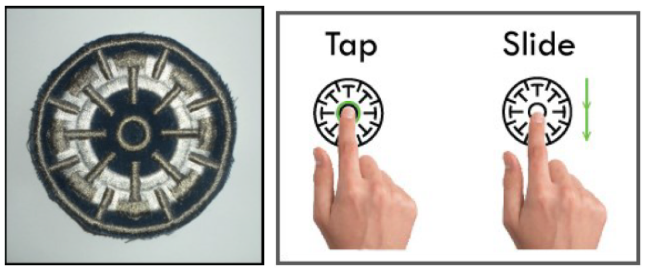
\includegraphics[width=\columnwidth]{jogwheel.png}
  \caption{\emph{Jogwheel} sensing surface textile}
\end{figure}
%
%
% here we can add everything to e-Textiles

Another type of e-textile is the one presented by SmartSleeve [ref], where the fabric is an input surface made alternating conductive and insulating textile bands. Then another pressure-sensible fabric is set under the first one, beneath wich there’s another fabric alternating conductive and non-conductive bands  orthogonal to the top layer. This allows to touch and register both the position and the intensity with a matrix representation. The sensor density is 1.66 sensors per square inch, which allows for a discrete sensor density. However, as the system is working with the short-circuit principle and the wires are not insulated, skin moisture can lead to false position sensing. To avoid that, the authors have put SmartSleeve over a long-sleeved running shirt. This solution, though, becomes unsuitable in summer for obvious reasons. %maybe better written
%
Project Jaquard [ref], instead, expoits a capacitive system where the fabric is one layer textile where some of the wires in the weft and warp are electrical wires. As the touch sensing is made with capacitance measure, this system is not vulnerable to skin moist false sensing. Different materials have been investigated to create the electrical wires, both for simplicity over the creation of the fabric and the necessity of flexibility needed for comfort. The material chosen is the copper because it has similar properties of others fabrics like cotton, silk and wool when the wire diameter is 50µm.
%
%
% At the end of this chapter we should discuss the advantages and disadvantages of the various technologies.
%


\section{Social acceptability of touch-based Wearables}
% In this part we should discuss the issues with social acceptability
% first in general
% second regarding the specific devices we presented in the showcase
% When developing body-worn controllers, two things have to be considered. On the one hand the body part where this technology is placed - on the other, the design of the technology so that the system adapts as well as possible to the selected body part. These two parameters are a basic requirement for the most user-friendly system. [Source: Don't Mind me Touching my wrist]. However, another parameter is crucial and will be discussed in more detail in this section - social acceptability.

Social acceptance includes the social competence and presentation in which people behave in such a way that they feel comfortable in society or do not embarrass themselves or draw attention to themselves. [13] (Source 13 of the paper Don't Mind me Touching my wrist -> SEARCH!). The use of portable technologies is therefore also subject to social conventions. The body-worn controllers listed in the previous sections are associated with new designs, new shapes and, above all, new interactions that might seem unfamiliar to third parties at first appearances.
An example of this is the Bluetooth headset from the early 2000s. At first, there was less acceptance in society because it looked as if the user was talking to himself. After a while, however, the Bluetooth headset became established in society. [24] (Source 24 of the paper Don't Mind me Touching my wrist SEARCH!). The use of body-worn controllers could initially lead to similar effects and acceptance problems, for which reason possible application examples are presented below, evaluated and discussed with the aid of current studies.

The perception of technology use in public spaces can be different in every culture, because the standards of social behaviour vary in many countries. [3] (Source: Dont mind me touching my wrist -> SEARCH). This also should be considered in the development of new interactive systems, which is why it also needs to be part of the research of social acceptance.  Campbell et al. have shown in their study on the public use of mobile phones, that there are indeed differences in this field. For example, Campbell et al. discovered that in Japan the use of mobile phones in buses or sidewalks is less accepted by society than in a restaurant. In many other cultures, this is rather the opposite. [Campbell, S. Perceptions of mobile phone use in public settings: a cross-cultural comparison. In Proc. of the Intl. Journal of Communication 1, (2007), 738-757.)]
These results lead to the conclusion that there are also cultural differences in perception when interacting with body-worn controllers which need to be explored.

Social acceptance includes various factors, which is why different methods are used to evaluate them. A handful of these methods will be mentioned and discussed in the next chapter.
[X] = [Profita, H. P., Clawson, J., Gilliland, S., Zeagler, C., Starner, T., Budd, J., \& Do, E. Y. L.
(2013, September). Don't mind me touching my wrist: a case study of interacting with on-body
technology in public. In
(pp. 89-96). ACM.]
Methods to review social acceptability
%
% During my research I stumbled upon various methods to review the social acceptability of wearables (testing devices in public, testing devices in labs, testing with functional devices, testing with dummies, interviews which were more like a conversation, interviews with a simple likert scale (1..5) … the list goes on)
% We should discuss these techniques - what are advantages, disadvantages? What methods are practical / necessary?

Since social acceptability is a major issue when it comes to the adaptation of new technology (Don’t mind my touching my wrist - page 90) there is also the need to measure it appropriately. Different researches have different approaches to review the social acceptability of their respective research.
\section{Testing - Demonstrating Technology}

\subsection{Testing with dummy (without working technology)}
% Belt (public), Usable Gestures, More Than Touch
One of the first possible way to study and discuss both comfort and easiness  to interact with clothing as an input is to interview people about what they would do to enact some commands on their skin. This is the main principle adopted by More Than Touch [ref], where the authors says: “This allowed us to observe participants’ unrevised behavior, free of the restrictions of current hardware. This method prove helpful in previous work for deriving implications for future hardware and system designs to accommodate this user behavior.”
These research types allow to have a common ground, as they help defining areas where the touching is not possible, either because it’s a position not easily acceptable or because it’s not a social acceptable position. Testing usually is done in a laboratory, like with Usable Gestures [ref], where the user feels less the social pressure given by the presence of many people. So this type of testing is quite useful when beginning the development of a technology, as it’s not related to the current hardware, but has some limitations both because it doesn’t consider the necessary tradeoffs that must be made to go from the idea of the device to the actual working device and because the laboratory itself doesn’t reflect the everyday situation that a person and a device will encounter on.

\subsection{Testing in private (lab situation)}
% Belt (working prototype), Pinstripe, Usable Gestures, More Than Touch, SmartSleeve
The main testing environment was the laboratory one, as it presents the optimal situation where on one side the subject is not distracted by other stimuli and it’s more focused on the topic he’s presented (in this case  gesture testing) and on the other side researchers can verify more data recorded by the sensor, receive voice feedback by testing subject, like what they’re doing, their mental model which explains why they’re doing this gesture, while they’re performing it. The first prototype shown is the Belt [ref], where users had a visual feedback for the belt-interaction, which was Google Glass. The main result, common to all interactions, is that the area reachable to the dominant hand is preferred. In the Belt case, in particular, the area which had a higher interaction density is the front of the belt, on the side of the dominant hand, where user expressed the easiness and comfortability of interacting with a body-worn device. The second case-study taken into account by this paper is the Pinstripe [ref] in which test subjects would perform gestures in three different context, which are sitting, standing still and walking, and  for each of them they’ll try to perform a grabbing gesture in all the sixteen areas of their body defined by the authors. For each of them they expressed the easiness and the personal acceptance of doing that gesture in that context. The most important discovery, found out also by the  papers [various ref] , is that the preferred part of the body is the upper side of the body, both for accessibility, which relates to easiness, and the comfort related to the social acceptance.
Moreover, as shown by [ref MoreThanTouch, Assessing the wearability and related] the mind model related to the touchscreen UI influences mostly the types of gestures (i.e. pinch to zoom is transferred from the smartphone to the textile surface)

\subsection{Testing in public}
% Belt (no working tech), Usable Gestures, Pinstripe
%
When transferring from the private laboratory environment to the public and social environment where the subject meets people who are looking to himself, some different aspects can be noticed: first of all, the area, that was shown as acceptable is reduced considerably and comprehend only the arm, the pocket area and the sternum [ref Pinstripe]. This can be related to the [ref More than touch] were people felt uncomfortable in area where they’re not used to touching. An example that we can make is the fact that in the pocket area one reaches it for his smartphone, wallet or keys, or in case of the forearm, usually one can look at his watch. One remark made in Pinstripe [ref], in fact, was that even though the sternum had a high rating, female testers were underlying that it would not be socially acceptable to interact in that area, so the areas where the input should be placed depends on cultural background, sex and personal attitude.

\subsection{Testing with device (working technology)}
% Belt (private), Pinstripe, Usable Gestures



\subsubsection{Demo video showing technology}
% Don’t mind Me, The Social Comfort, Usable Gestures
The paper "Don't Mind Me Touching My Wrist: A Case Study of Interacting with On-Body Technology in Public" deals with the social acceptability of on-body technology and examines which cultural differences of perception can arise during interaction with an e-textile. [x] The USA and South Korea were chosen as reference countries for this purpose. In order to investigate perception, the “Jogwheel” was used, which we have already discussed above. The use case was the control of a mobile phone, to be exact, muting it after an incoming call, during a four eye conversation in an elevator. The scenario was simulated twice in each of the two countries - once the interaction with the jogwheel was done by a woman and once by a man. This was recorded by camera and then the video was presented to the participants in an online-survey. This allows evaluation of the scenarios in public context. The video was shown to the participants once with a view from a distance (~1.2-1.5 meters) and once with a focus on the interaction (distance ~30-45 centimeters)). After the videos, various questions  about the perception of the interaction with the jogwheel were raised. %TODO - List results of survey - i will do until Sunday (Philipp U.)



Interviews:

Questions based on a likert scale (or multiple choice based interviews in general)
Belt (focus on likert), Don’t mind me (focus on multiple choice), Pinstripe (1. study), The Social Comfort, Usable Gestures (first study)

Interviews structured like a conversation
Belt, Don’t mind me, Pinstripe (2. study), The Social Comfort, Usable Gestures (2. study), More than touch

\section{Second section in another file}
Even if the file is different, using the
\begin{verbatim}
  \section{Second section in another file}
Even if the file is different, using the
\begin{verbatim}
  \section{Second section in another file}
Even if the file is different, using the
\begin{verbatim}
  \include{anotherSection}
\end{verbatim}
we can add the text in the main file.

\end{verbatim}
we can add the text in the main file.

\end{verbatim}
we can add the text in the main file.

\bibliographystyle{SIGCHI-Reference-Format}
 % \bibliography{File.bib}

\end{document}

%%% Local Variables:
%%% mode: latex
%%% TeX-master: t
%%% End:
